\documentclass{article}
\usepackage{graphicx}
\usepackage[T1]{fontenc}
\usepackage[utf8]{inputenc}
\usepackage[italian]{babel}
\usepackage{amsmath}
\usepackage{todonotes}
\usepackage{float}
\usepackage[absolute,overlay]{textpos}
\usepackage{enumitem}
\usepackage{pdfpages}
\usepackage{subfigure}
\usepackage{hyperref}
\usepackage{multirow}
\usepackage{booktabs}
\usepackage[table]{xcolor}
\usepackage[margin=2.0cm]{geometry}
\usepackage{ upgreek }
\usepackage{wrapfig}
\usepackage{lipsum} % Per testo fittizio


\title{\textbf{Pendolo a torsione}}
\author{\textbf{Gruppo 03}\\Zoya Veronese\qquad2145523\qquad zoya.veronese@studenti.unipd.it\\ Leonardo Melis\qquad 2148583\qquad leonardo.melis@studenti.unipd.it\\ Gianluca Nichetti\qquad 2137786\qquad  gianluca.nichetti@studenti.unipd.it}
\date{15 giugno 2025}

\begin{document}
\maketitle

\section{Abstract}
L'esperienza ha l'obiettivo di verificare sperimentalmente il comportamento di un oscillatore armonico smorzato e forzato e di trovarne la frequenza e l'ampiezza di risonanza mediante l'utilizzo di un pendolo a torsione. Il sistema è soggetto a una coppia torcente generata da un motorino e a una forza di smorzamento dovuta all’interazione con un liquido viscoso. Per una stima più accurata dei parametri del sistema la curva sperimentale è stata interpolata con un fit lorentziano. La procedura prevede l'acquisizione delle oscillazioni angolari mediante un sensore, per diverse frequenze forzanti da 0.85 a 1.50 Hz. L'esperienza inoltre ha lo scopo di stimare il coefficiente di smorzamento del liquido in cui é immersa la massa, mediante lo studio delle oscillazioni dopo l'interruzione della forzante.

\section{Introduzione teorica}
Il pendolo a torsione rappresenta un classico esempio di oscillatore armonico rotazionale, in cui una massa rigida è sospesa tramite un filo elastico soggetto a deformazione torsionale. Nel caso ideale di oscillazioni libere e non smorzate, il moto del pendolo a torsione è descritto dall’equazione differenziale del secondo ordine:
\begin{equation*}
    I_z \ddot{\theta} + k \theta = 0
\end{equation*}
 nella quale $I_z$ è il momento d’inerzia della massa rispetto all’asse di rotazione,
k è la costante di torsione del filo, $\theta$ è la coordinata angolare. La soluzione è un moto armonico semplice con pulsazione naturale 
\begin{equation*}
    \omega_0 = \sqrt{\frac{k}{I_z}}
\end{equation*}
Tuttavia è necessario considerare l’effetto di forze dissipative, tipicamente attrito viscoso, con un momento torcente dissipativo proporzionale alla velocità angolare: $-b\omega$; nella quale $b$ è coefficiente di smorzamento. L’equazione del moto diventa quindi:
\begin{equation*}
    I_z \ddot{\theta} + 2\beta \dot{\theta} + k \theta = 0
\end{equation*}
La soluzione di questa equazione descrive un moto armonico smorzato, in cui l’ampiezza delle oscillazioni decresce esponenzialmente nel tempo. In particolare, la pulsazione del sistema smorzato è $\omega_s=\sqrt{\omega_0^2-(\frac{b}{2I_z})^2}$, evidenziando come lo smorzamento modifichi la dinamica del sistema.\\
Se al sistema viene applicata una forza torcente esterna periodica, ad esempio generata da un motorino, il moto risulta descritto dalla seguente equazione non omogenea:
\begin{equation}
    I_z \ddot{\theta} + 2\upgamma \dot{\theta} + k \theta = \tau_0 \cos(\omega t+\phi)\qquad \upgamma=\frac{2\beta}{I_z}
\end{equation}
 nella quale $\tau_0$ è l’ampiezza del momento torcente esterno e $\omega$ la sua pulsazione. La soluzione generale di questa equazione è costituita da due contributi: il moto transitorio, che si estingue nel tempo a causa dello smorzamento, e il moto stazionario forzato, assume la forma:
\begin{equation}
    \theta(t) = \theta_{0,s} e^{-\upgamma t} \cos(\omega_{s} t +\phi)+ \theta_{0,f}\cos(\omega_{f} t + \phi)
\end{equation}
  Il primo membro rappresenta la fase transitoria, mentre il secondo quella permanente.\\L'ampiezza $\theta_0$ del moto forzato dipende dalla frequenza di eccitazione e mostra un massimo in corrispondenza della frequenza di risonanza, che per sistemi debolmente smorzati è approssimativamente:
\begin{equation*}
    \theta_{0,f}= \frac{\frac{\tau_{0,f}}{I_z}}{\sqrt{(\omega_0^2-\omega_f^2)^2+4\upgamma ^2 \omega_f^2}}
\end{equation*}
Il fenomeno di risonanza si manifesta quindi quando la frequenza della forza esterna si avvicina a quella naturale del sistema, provocando un’amplificazione dell’ampiezza di oscillazione. Il picco di risonanza è tanto più acuto quanto minore è lo smorzamento.\\
La curva di risonanza, che rappresenta l’ampiezza in funzione della frequenza forzante, ha un profilo tipicamente descritto da una funzione di tipo Lorentziano ( fare riferimento alla formula 10 in appendice):
\begin{equation}
L(x) = \frac{A}{(B^2+2C^2 - x^2)^2 + 4C^2 x^2}
\end{equation}
L’interpolazione sperimentale tramite un fit lorenziano consente di estrarre con precisione i parametri dinamici fondamentali: pulsazione naturale, smorzamento e costante torcente.

\section{Metodologia e apparato strumentale}
\begin{wrapfigure}{R}{0.3\textwidth}
  \centering
  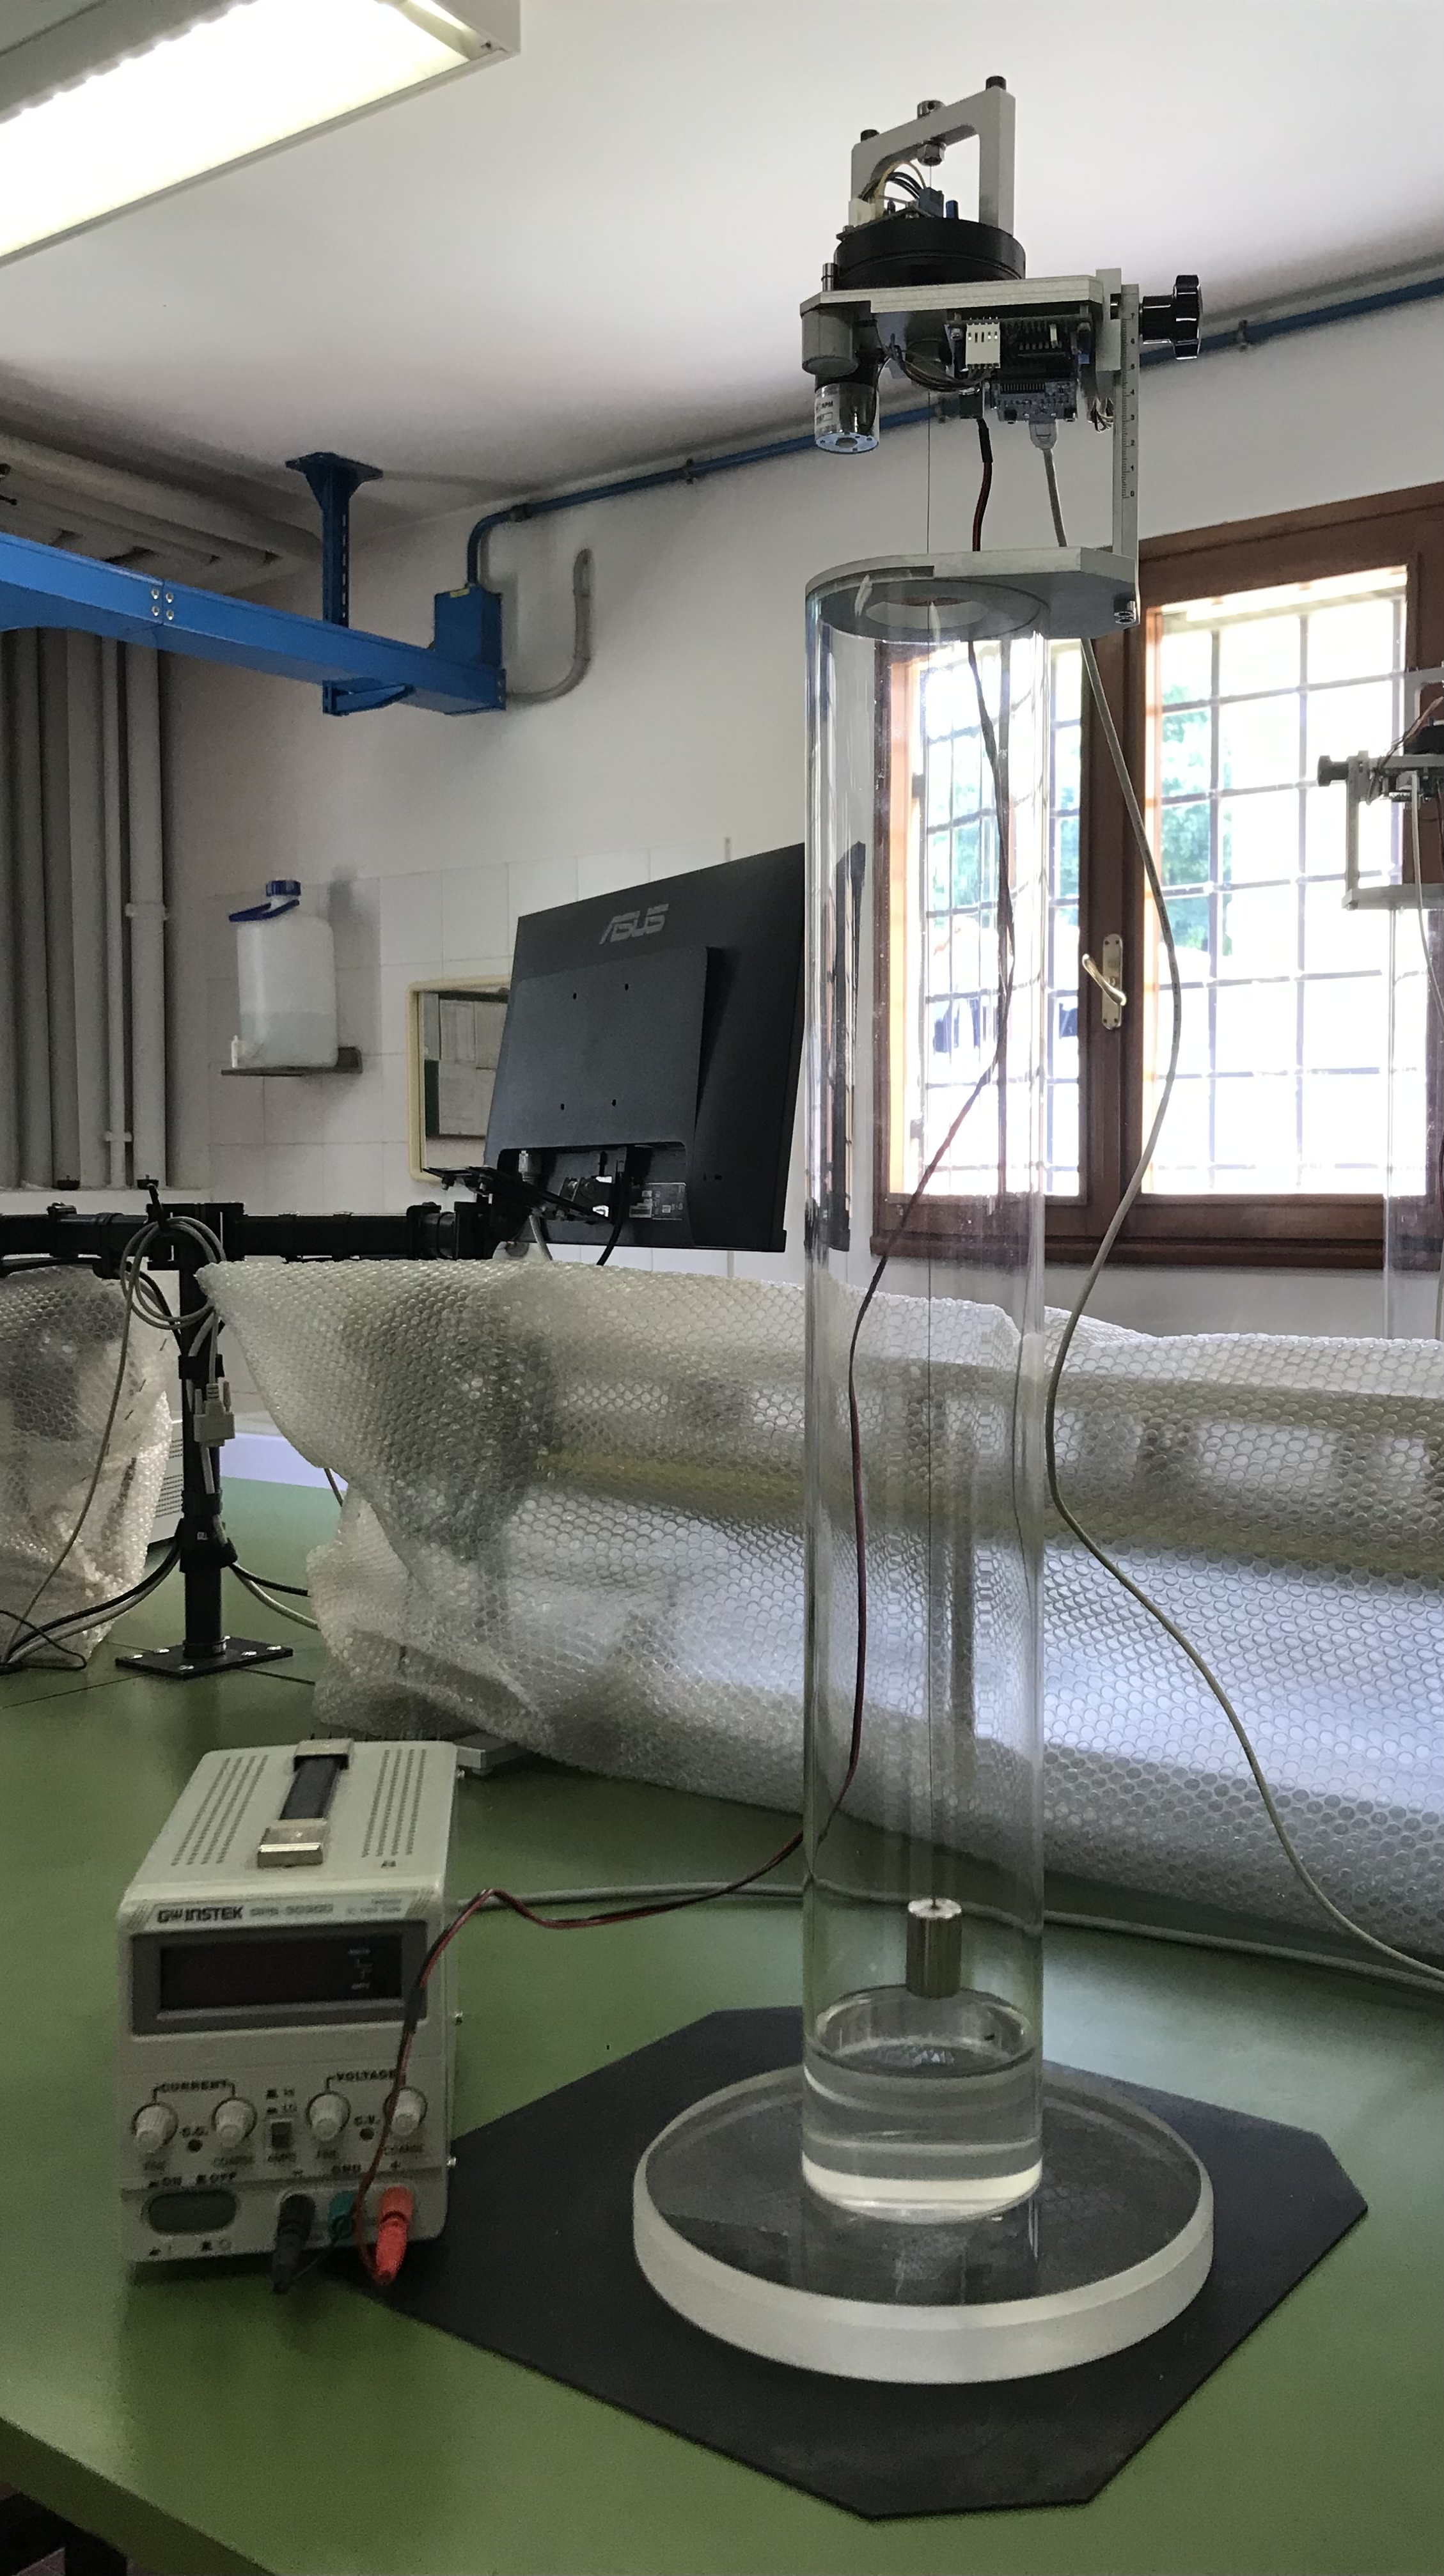
\includegraphics[width=0.28\textwidth]{Strumento.jpeg}
  \caption{Foto apparato strumentale}
\end{wrapfigure} 

L’apparato sperimentale utilizzato per lo studio della risonanza in un pendolo a torsione è costituito da un sistema meccanico e da una strumentazione elettronica per l’acquisizione e l’analisi dei dati. Il sistema oscillante è composto da un pendolo a torsione, realizzato con una massa cilindrica in acciaio solidamente connessa a un filo sottile di acciaio armonico. La massa ha le seguenti caratteristiche geometriche e fisiche: massa $115.5\pm0.1g$, diametro $22.7\pm0.1mm$ e altezza $34.01\pm0.1mm$. Il filo ha una lunghezza approssimativa di 75 cm e un diametro di circa 0.4 mm.
Il moto del pendolo è forzato mediante un motorino elettrico che applica un momento torcente periodico regolabile in frequenza. Per introdurre un effetto dissipativo, il sistema è immerso in un liquido smorzante.
Il rilevamento delle oscillazioni angolari è affidato a un sensore che misura la coordinata angolare $\theta$ in funzione del tempo. I dati sono acquisiti con una scheda di acquisizione temporale avente una risoluzione temporale di 0.02 s. L’intervallo di frequenze forzanti esplorate va da 0.90Hz a 1.00Hz. I valori registrati per ciascuna frequenza comprendono il tempo, l’ampiezza della forzante mantenuta costante per tutte le misure a 12 millesimi di giro, e l’ampiezza dell’oscillazione misurate in giri.
\\
Le misurazione sono state effettuate mediante tale procedura: innanzi tutto si è immersa la massa all'interno del liquido, successivamente si è attivata la forzante e, raggiunta un'oscillazione stabile, si è cominciato a raccogliere i dati di tempo, forzante e ampiezza delle oscillazioni. Dopo 5min dall'inizio della raccolta dati la forzante viene interrotta e si lascia che l'attrito viscoso del fluido smorzi la torsione per alcuni minuti. Nelle serie di misurazioni effettuate il primo giorno di laboratorio (con frequenza della forzante 0.90, 1.00, 0.99, 0.98 e 0.97Hz) si è lasciato oscillare il pendolo a torsione fino a 5min dopo l'interruzione della forzante. Per le altre serie, effettuate in un giorno successivo si è deciso di lasciar oscillare il pendolo solamente per 2 min dopo l'interruzione della forzante, in quanto, nella seconda parte della misurazione, se nell'analisi dati si utilizzano misurazioni con oscillazioni molto piccole é più probabile commettere un'errore maggiore nella stima dei parametri del fit.

\newpage
\section{Risultati}
\subsection{Frequenza di risonanza}
Graficando le misure raccolte è emerso chiaramente che le oscillazioni del pendolo non sono centrate sullo zero, ma presentano un offset variabile da una serie all'altra; infatti, nella prima giornata tale offset è mediamente negativo, mentre nella seconda risulta positivo e molto più evidente.

\begin{figure}[H]
    \centering
    \subfigure{
\includegraphics[width=0.90\textwidth]{/home/nichettg/Codici/Laboratorio/8.PendoloTorsione/Images/ConfrontoForzanti.pdf}}
    \caption{Confronto delle serie alla stessa frequenza della prima giornata (sopra) e della seconda (sotto). Data l'evidente discrepanza delle misure, si è deciso di mantenere separate nell'analisi dati le serie raccolte nei due giorni.}
\end{figure}

\begin{figure}[h!]
    \centering
    \subfigure{
\includegraphics[width=0.90\textwidth]{/home/nichettg/Codici/Laboratorio/8.PendoloTorsione/Images/ConfrontoMassimi.pdf}}
  \caption{Confronto degli estremi corretti e grezzi nelle serie alla stessa frequenza: sopra la prima giornata, sotto la seconda}
\end{figure}

In seguito, per trovare massimi e minimi, l'intera serie è stata suddivisa in intervalli di raggio $r$ tali che ciascun intervallo comprendesse un massimo e un minimo:

\begin{equation}
    r = \frac{\tau}{2} \upnu
\end{equation}

nella quale $\tau$ è il periodo, ovvero l'inverso della frequenza della forzante, e $\upnu$ è la frequenza di campionamento dei dati, cioè 50Hz.
Ai valori degli estremi locali così individuati è stato applicato un fattore di correzione pari al valore medio dell’offset dei dati nella serie stessa, calcolato come la media dei dati raccolti. Assumendo che i campioni dei massimi e dei minimi seguano una distribuzione gaussiana, in quanto non presentano alcun tipo di distribuzione anomala che possa suggerire una sistematica strumentale, sono state calcolate separatamente le loro medie. L'ampiezza media corretta è stata quindi determinata come la media aritmetica delle due medie.


\begin{table}[H]
\small
\centering
\begin{tabular}{|c|c|c|c|c|}
\toprule
\textbf{Serie} & \textbf{Media massimi (rad)} & \textbf{Media minimi (rad)} & \textbf{Ampiezza corretta (rad)} & \textbf{Ampiezza grezza (rad)} \\
\midrule
$0.9\,\text{Hz}$ & $(3.00 \pm 0.02) \times 10^{-1}$ & $(-2.10 \pm 0.02) \times 10^{-1}$ & $(2.52 \pm 0.03) \times 10^{-1}$ & $(2.55 \pm 0.03) \times 10^{-1}$ \\
$0.97\,\text{Hz}$ & $(1.45 \pm 0.01)$ & $(-1.39 \pm 0.01)$ & $(1.42 \pm 0.01)$ & $(1.42 \pm 0.01)$ \\
$0.98\,\text{Hz}$ & $(9.2 \pm 0.2) \times 10^{-1}$ & $(-8.7 \pm 0.1) \times 10^{-1}$ & $(8.94 \pm 0.01) \times 10^{-1}$ & $(8.95 \pm 0.02) \times 10^{-1}$ \\
$0.99\,\text{Hz}$ & $(6.3 \pm 0.2) \times 10^{-1}$ & $(-5.8 \pm 0.1) \times 10^{-1}$ & $(6.07 \pm 0.02) \times 10^{-1}$ & $(6.06 \pm 0.03) \times 10^{-1}$ \\
$1\,\text{Hz}$ & $(5.5 \pm 0.2) \times 10^{-1}$ & $(-4.2 \pm 0.2) \times 10^{-1}$ & $(4.85 \pm 0.03) \times 10^{-1}$ & $(4.84 \pm 0.04) \times 10^{-1}$ \\
\midrule
$0.91\,\text{Hz}$ & $(2.9 \pm 0.2) \times 10^{-1}$ & $(-2.9 \pm 0.1) \times 10^{-1}$ & $(2.93 \pm 0.01) \times 10^{-1}$ & $(6.69 \pm 0.10) \times 10^{-1}$ \\
$0.92\,\text{Hz}$ & $(3.5 \pm 0.1) \times 10^{-1}$ & $(-3.6 \pm 0.1) \times 10^{-1}$ & $(3.57 \pm 0.01) \times 10^{-1}$ & $(5.9 \pm 0.2) \times 10^{-1}$ \\
$0.93\,\text{Hz}$ & $(4.6 \pm 0.2) \times 10^{-1}$ & $(-4.7 \pm 0.2) \times 10^{-1}$ & $(4.64 \pm 0.01) \times 10^{-1}$ & $(5.29 \pm 0.02) \times 10^{-1}$ \\
$0.94\,\text{Hz}$ & $(6.6 \pm 0.2) \times 10^{-1}$ & $(-6.6 \pm 0.2) \times 10^{-1}$ & $(6.57 \pm 0.01) \times 10^{-1}$ & $(6.57 \pm 0.02) \times 10^{-1}$ \\
$0.95\,\text{Hz}$ & $(1.11 \pm 0.02)$ & $(-1.13 \pm 0.02)$ & $(1.119 \pm 0.001)$ & $(1.12 \pm 0.02)$ \\
$0.955\,\text{Hz}$ & $(1.66 \pm 0.01)$ & $(-1.64 \pm 0.01)$ & $(1.648 \pm 0.001)$ & $(1.65 \pm 0.04)$ \\
$0.9575\,\text{Hz}$ & $(1.95 \pm 0.01)$ & $(-1.93 \pm 0.02)$ & $(1.94 \pm 0.01)$ & $(1.94 \pm 0.04)$ \\
$0.96\,\text{Hz}$ & $(2.00 \pm 0.03)$ & $(-2.00 \pm 0.02)$ & $(1.998 \pm 0.002)$ & $(2.00 \pm 0.01)$ \\
$0.96125\,\text{Hz}$ & $(2.15 \pm 0.01)$ & $(-2.09 \pm 0.01)$ & $(2.121 \pm 0.002)$ & $(2.12 \pm 0.04)$ \\
$0.96183\,\text{Hz}$ & $(2.15 \pm 0.01)$ & $(-2.06 \pm 0.02)$ & $(2.105 \pm 0.002)$ & $(2.11 \pm 0.04)$ \\
$0.9625\,\text{Hz}$ & $(2.09 \pm 0.01)$ & $(-2.06 \pm 0.01)$ & $(2.077 \pm 0.001)$ & $(2.08 \pm 0.04)$ \\
$0.965\,\text{Hz}$ & $(1.89 \pm 0.02)$ & $(-1.86 \pm 0.02)$ & $(1.872 \pm 0.001)$ & $(1.87 \pm 0.04)$ \\
$0.97\,\text{Hz}$ & $(1.40 \pm 0.01)$ & $(-1.32 \pm 0.01)$ & $(1.361 \pm 0.002)$ & $(1.36 \pm 0.04)$ \\
\bottomrule
\end{tabular}
\caption{Medie di massimi e minimi corretti e ampiezze corrette e grezze per ogni serie. Le prime cinque righe corrispondono al Giorno 1, le successive al Giorno 2.}
\label{max_min_amp_scientifica}
\end{table}


%\begin{figure}[h!]
%    \centering
%    \includegraphics[width=0.75\linewidth]{confronto_massimi_esempio.jpg}
%    \caption{Grafico di confronto tra estremi corretti e grezzi nella serie più vicina alla frequenza di risonanza (2° giornata)}
%    \label{fig:enter-label}
%\end{figure}

Successivamente, per ricavare la frequenza di risonanza, è stato eseguito un fit Lorentziano (formula 10 in appendice) sulle ampiezze dell'oscillazione ricavate dalla soluzione particolare dell'equazione del moto del pendolo (formula seguente):

\begin{equation}
    \upvartheta_{part}(\omega_f) = \frac{A}{\sqrt{(\omega_R^2 + 2\gamma^2 - \omega_f^2)^2 + 4\gamma^2 \omega_f^2}}
\end{equation}

nella quale $\omega_f$ è la pulsazione della forzante, $A$ è l'ampiezza della forzante, $\omega_R$ è la pulsazione di risonanza e $\gamma$ è il coefficiente di smorzamento.
\\
Dividendo $\omega_R$ per $2\pi$ si sono ottenute due diverse frequenze di risonanza, una ricavata dalle misure della prima giornata e l'altra da quelle della seconda; e inoltre sempre tramite la curva Lorentziana è stata ricavata l'ampiezza corrispondente alla frequenza di risonanza.

\begin{table}[h!]
    \centering
    \begin{tabular}{llr}
      \toprule \hline
      & Giorno 1 & Giorno 2 \\
      \midrule
      Frequenza ($\mathcal{V}_R$) & $(9645.8 \pm 1.4) \times 10^{-4}Hz$ & $(961035 \pm 6) \times 10^{-6}Hz$ \\
      \midrule
      Ampiezza & $(1.600 \pm 0.009) rad$ & $(2.121 \pm 0.005) rad$ \\
      \bottomrule
    \end{tabular}
    \caption{Confronto frequenze di risonanza e ampiezze alla $\mathcal{V}_R$ delle due giornate}
    \label{confronto_risonanza}
\end{table}

\subsection{Coefficiente di smorzamento}
Per calcolare il coefficiente di smorzamento, sono stati considerati solo gli estremi locali rilevati dopo lo spegnimento della forzante. Poiché il moto in questa fase è un moto armonico smorzato, è stato applicato il logaritmo naturale a entrambi i membri dell’equazione per linearizzare la relazione:

\begin{equation}
    A(t)= A_0 e^{-\gamma t} \Rightarrow lnA(t)=lnA_0-\gamma t
\end{equation}
con $\gamma$ coefficiente di smorzamento.


In seguito è stato eseguito un fit lineare con la precedente relazione dal quale sono stati ricavati i valori di $\gamma$ per ognuna delle serie. Come si può notare dal grafico Fig. 4, i dati risultano sempre meno lineari con l'avanzare del tempo. E' stato quindi calcolato il coefficiente di Pearson (formula 15 in appendice) fino ad un certo indice dei dati e, facendo variare questo indice in un range tra 1/10 e 1, si è trovato il valore per cui il coefficiente di Pearson risultava migliore rispetto all'ipotesi di anticorrelazione lineare totale (quindi coefficiente uguale a meno uno). Per valutare la compatibilità è stato eseguito un test di Student a una coda (in appendice sono riportati i valori dei p-value risultanti e gli intervalli scelti per il fit per ogni serie). Nei casi in cui siano risultati compatibili i coefficienti di Pearson calcolati per piu indici diversi (ad esempio 1/10, 2/10 e 3/10) si è scelto l'indice maggiore per garantire una maggiore numerosità del campione. sia  Il coefficiente di smorzamento $\gamma$ era già stato calcolato anche con il fit Lorentziano di cui alla $(5)$.

\begin{table}[h!]
\centering
\begin{tabular}{cc}
\toprule
\multicolumn{2}{c}{\textbf{Misure del coefficiente $\gamma$ [rad/s]}} \\
\midrule
\textbf{Giorno 1} & \textbf{Giorno 2} \\
\midrule
$(6.62 \pm 0.02) \times 10^{-2}$ & $(4.472 \pm 0.005) \times 10^{-2}$\\
\bottomrule
\end{tabular}
\caption{Valori misurati del coefficiente $\gamma$ e relativa incertezza $\sigma_\gamma$ con fit Lorentziano}
\label{tab:gamma_pm_lorentz}
\end{table}

%----------------------------------------------------------------------
\begin{table}[H]
\centering
\small % Riduce il font per farle stare tutte
\begin{minipage}{0.31\textwidth}
\centering
\textbf{Giorno 1}\\[0.5ex]
\begin{tabular}{cc}
\toprule
\textbf{Serie} & $\gamma \pm \sigma_\gamma$ [rad/s] \\
\midrule
$0.90\,\text{Hz}$ & $(42.1 \pm 1.2)\!\times\!10^{-3}$ \\
$0.97\,\text{Hz}$ & $(452.5 \pm 2.4)\!\times\!10^{-4}$ \\
$0.98\,\text{Hz}$ & $(423.8 \pm 4.1)\!\times\!10^{-4}$ \\
$0.99\,\text{Hz}$ & $(381.2 \pm 6.5)\!\times\!10^{-4}$ \\
$1.00\,\text{Hz}$ & $(39.0 \pm 1.5)\!\times\!10^{-3}$ \\
\bottomrule
\end{tabular}
\end{minipage}
\hfill
\begin{minipage}{0.31\textwidth}
\centering
\textbf{Giorno 2}\\[0.5ex]
\begin{tabular}{cc}
\toprule
\textbf{Serie} & $\gamma \pm \sigma_\gamma$ [rad/s] \\
\midrule
$0.91\,\text{Hz}$ & $(47.0 \pm 1.6)\!\times\!10^{-3}$ \\
$0.92\,\text{Hz}$ & $(38.4 \pm 1.9)\!\times\!10^{-3}$ \\
$0.93\,\text{Hz}$ & $(369.9 \pm 9.1)\!\times\!10^{-4}$ \\
$0.94\,\text{Hz}$ & $(423.3 \pm 5.5)\!\times\!10^{-4}$ \\
$0.95\,\text{Hz}$ & $(461.8 \pm 1.8)\!\times\!10^{-4}$ \\
$0.955\,\text{Hz}$ & $(465.5 \pm 1.6)\!\times\!10^{-4}$ \\
$0.9575\,\text{Hz}$ & $(392.7 \pm 2.5)\!\times\!10^{-4}$ \\
\bottomrule
\end{tabular}
\end{minipage}
\hfill
\begin{minipage}{0.31\textwidth}
\centering
\textbf{Giorno 2}\\[0.5ex]
\begin{tabular}{cc}
\toprule
\textbf{Serie} & $\gamma \pm \sigma_\gamma$ [rad/s] \\
\midrule
$0.96\,\text{Hz}$ & $(474.1 \pm 1.7)\!\times\!10^{-4}$ \\
$0.96125\,\text{Hz}$ & $(477.5 \pm 1.9)\!\times\!10^{-4}$ \\
$0.96183\,\text{Hz}$ & $(468.9 \pm 1.5)\!\times\!10^{-4}$ \\
$0.9625\,\text{Hz}$ & $(463.3 \pm 2.1)\!\times\!10^{-4}$ \\
$0.965\,\text{Hz}$ & $(472.8 \pm 1.5)\!\times\!10^{-4}$ \\
$0.97\,\text{Hz}$ & $(460.9 \pm 2.4)\!\times\!10^{-4}$ \\
\bottomrule
\end{tabular}
\end{minipage}

\caption{Valori misurati di $\gamma$ e incertezza $\sigma_\gamma$ con il metodo della linearizzazione}
\label{tab:gamma_tripla}
\end{table}
%----------------------------------------------------------------------

\begin{figure}[h!]
    \centering
    \subfigure{
\includegraphics[width=0.70\textwidth]{/home/nichettg/Codici/Laboratorio/8.PendoloTorsione/Images/ConfrontoSmorzati.pdf}}
  \caption{Confronto del moto smorzato (con correzione di offset già applicata): sopra la prima giornata, sotto la seconda}
\end{figure}

\begin{figure}
    \centering
    \subfigure{
\includegraphics[width=0.70\textwidth]{/home/nichettg/Codici/Laboratorio/8.PendoloTorsione/Images/ConfrontoMassimiSmorzamento.pdf}}
    \caption{Confronto dell'ampiezza linearizzata delle serie alla stessa frequenza (0.97Hz), con la prima giornata sopra e la seconda sotto e $\gamma=-b$. È doveroso sottolineare che il p-value del test del $\chi^2$ (riportato nella legenda) è molto piccolo in entrambi i casi, ciò implica che questa linearizzazione non è una rappresentazione accurata dei dati probabilmente a causa di una sottostima delle incertezze. }
\end{figure}

Il valore estremamente basso del p-value del test del $\chi^2$ relativo alla bontà del fit evidenzia come i dati non vengano rappresentati bene dall'approssimazione lineare calcolata. Valutando infatti anche i coefficienti di Pearson (riportati in appendice) si può vedere che, anche se risultano compatibili con una significanza di 0.05, essi si discostano comunque dal valore ipotizzato di meno uno. Questa discrepanza è probabilmente dovuta a delle incertezze sperimentali molto basse.

%-------------------------------------------------------------------------------------------------------
\section{Discussione dei risultati}
\subsection{Confronto di risultati}
\begin{figure}[H]
    \centering
    
\includegraphics[width=0.90\linewidth]{/home/nichettg/Codici/Laboratorio/8.PendoloTorsione/Images/Lorentziana.pdf}
    \caption{Confronto Lorentziane del primo e del secondo giorno }
    \label{fig:enter-label}
\end{figure}
\begin{table}[h!]
    \centering
    \begin{tabular}{ccc}
     \textbf{Parametro del fit} & \textbf{Giorno 1}    &\textbf{Giorno 2} \\
      A   &$(1285\pm8)\times10^{-3} rad$  & $(1146\pm1)\times10^{-3} rad$\\ 
      B   &$(60606\pm9)\times10^{-4} rad/s$  & $(603836\pm4)\times10^{-5} rad/s$\\ 
      C   &$(6630\pm20)\times10^{-5} rad/s$  & $(4472\pm5)\times10^{-5} rad/s$\\ 
    \end{tabular}
    \caption{Parametri del fit Lorentziano (formula 10 in appendice).}
    \label{tab:my_label}
\end{table}
\begin{figure}[H]
    \centering
    
\includegraphics[width=1\linewidth]{/home/nichettg/Codici/Laboratorio/8.PendoloTorsione/Images/ConfrontoGamma.pdf}
    \caption{Confronto dei $\gamma$ ricavati. Gamma giorno 1 e gamma giorno 2 rappresentano i parametri stimati dal fit Lorentziano, giorno 1 e giorno 2 i valori ricavati dal fit lineare per ciascuna serie e la media invece è ricavata da tutti i valori (di entrambi i giorni) ricavati dai fit lineari. }
    \label{fig:enter-label}
\end{figure}

Dai dati emerge una forte incompatibilità tra le stime della frequenza di risonanza del primo e del secondo giorno (Fig.5), infatti, effettuando un test di compatibilità semplice (formula 13 in appendice) si ottiene che, nonostante i due valori non si discostino molto l'uno dall'altro sono incompatibili oltre i 23 $\sigma$. Effettuare un test di student in tale situazione non avrebbe portato ad alcuna conclusione perché, dato l'elevatissimo numero di misure raccolte, il numero di gradi di libertà sarebbe comunque stato molto alto. Si registra un incompatibilità ancor maggiore per quanto riguarda l'ampiezza di risonanza, infatti le due misure sono incompatibili oltre 50 $\sigma$, le misurazioni del secondo giorno riportano ampiezze notevolmente maggiori rispetto a quelle del primo specialmente nella porzione del picco, invece proseguendo verso le code le due curve tendono a congiungersi.\\Anche i coefficienti di smorzamento, ricavati dai fit Lorentziani, risultano fortemente incompatibili (oltre i 100 $\sigma$). Però, come si può osservare dal grafico di confronto (Fig.6), ad esclusione della stima Lorentziana del secondo giorno le altre stime sono locate in un intervallo compreso tra 0.035 e 0.05$rad/sec$; ed effettuando un test di compatibilità tra la media (linea tratteggiata in blu nella Fig.4) e la stima Lorentziana del primo giorno otteniamo un possibile compatibilità a 2.4$\sigma$. È importante però porre in evidenza che tale compatibilità è maggiormente dovuta al contributo dell'incertezza della media ($5\times10^{-4}$Hz) 10 volte maggiore di quella della stima Lorentziana ($5\times10^{-5}$Hz).
\begin{table}[H]
    \centering
    \begin{tabular}{|c|c|c|}
        \hline
        \multicolumn{2}{|c|}{Grandezze confrontate} & $\sigma$ \\ \hline 
        Frequenza di risonanza 1: $(9646 \pm 1) \times 10^{-4}\,\text{Hz}$ & Frequenza di risonanza 2: $(961035 \pm 6) \times 10^{-6}\,\text{Hz}$ & $23\sigma$\\ \hline 
        $\upgamma$ Lorentziano 1: $(4.472 \pm 0.005) \times 10^{-2}rad/s$ & $\upgamma$ Lorentziano 2: $(6.62 \pm 0.02) \times 10^{-2}rad/s$ & $104\sigma$ \\ \hline 
        $\upgamma$ Lorentziano 1: $(4.472 \pm 0.005) \times 10^{-2}rad/s$ & $\upgamma$ medio: $(4.35 \pm 0.05) \times 10^{-2}rad/s$ & $2.4\sigma$ \\ \hline 
        Ampiezza 1:$(1.600 \pm 0.009)rad$  & Ampiezza 2:$(2.121 \pm 0.005)rad$  & $51\sigma$ \\ \hline 
    \end{tabular}
    \caption{Tabella riassuntiva delle compatibilità}
    \label{tab:my_label} 
\end{table}

Data questa osservazione è legittimo dubitare dell'accuratezza dei parametri ricavati dalla Lorentziana del giorno 2 e quindi favorire i risultati ricavati dalla prima, anche l'incompatibilità dei parametri A e B sembra accreditare tale tesi ma per scartare con un buon grado di confidenza i dati ricavati da tale interpolazione sarebbe necessario  raccogliere altre misurazioni ed effettuare ulteriori test.
\subsection{Possibili cause di incompatibilità}
In ogni caso, nonostante non sia possibile scartare a priori la Lorentziana del secondo giorno è possibile ipotizzare delle ragioni per cui i valori presentano significative differenze.\\Innanzitutto il pendolo a torsione è uno strumento molto delicato che rischia di perdere la taratura alla minima perturbazione, oltre a non aver effettuato una taratura ogni presa dati non è stato possibile effettuare le misurazioni in un ambiente privo di agenti esterni che possono aver modificato la naturale oscillazione del pendolo. \\È stato ipotizzato che un altro fattore che può aver causato differenze nella stima di $\upgamma$nel primo e nel secondo giorno è la temperatura dell'ambiente che tra il primo e il secondo giorno è aumentata di circa 5C°. Quest'ipotesi però è stata successivamente scartata in quanto quest'aumento della temperatura non sarebbe stato sufficiente a far variare così tanto il coefficiente di smorzamento del liquido*.
\footnote{*fonte: Journal of Research of the National Bureau of Standards, Absolute Viscosity of Water at 20° C, 1. F. Swindellsr 1. R. Coer Jr. r and T. B. Godfrey  }
\\Un'altra possibile causa dell'incompatibilità può essere un'eventuale correlazione dei dati non tenuta in considerazione: i periodi sono uno successivo all'altro, il fatto che siano consecutivi implica che se il primo è sfasato lo sarà anche il secondo e così via. In tal caso sarebbe necessario stimare un coefficiente di correlazione che andrebbe ad influire nelle incertezze delle misurazioni aumentandole, dato che mediamente le incertezze ricavate sono molto piccole ,sempre inferiori all'1\% (formula per la propagazione delle incertezze, 14 in appendice).

\section{Conclusione}
In conclusione è possibile affermare che i nostri dati sono in accordo con le ipotesi teoriche infatti risultano valori di frequenza di risonanza, ampiezza di risonanza e coefficiente di smorzamento  accettabili che rientrano nel dominio naturale dei parametri fisici. Tuttavia non è stato possibile fornire una stima unica sufficientemente accurata a causa delle anomalie riscontrate nell'analisi dati; perciò è stato scelto di presentare due stime per ciascun obiettivo: frequenza di risonanza e ampiezza di risonanza (risultati riportati nella Tab.2) e coefficiente di smorzamento (risultati riportati nella Tab.3). Come già discusso precedentemente lo studio poteva essere implementato prestando maggior accortezza ad evitare la correlazione fra i dati raccolti ed effettuando le misurazioni in un ambiente più favorevole (privo di disturbi) e valutando tramite test specifici quali sono i fattori che influenzano l'accuratezza della misura. 

\newpage
\section{Appendice}
\subsection{Formule}
\begin{enumerate}
    \item Media pesata
\[
\bar{x} = \frac{\sum_{i=1}^{n} (\frac{x_i}{s_i^2})}{\sum_{i=1}^{n}(\frac{1}{s_i})^2}
\]
    \item Incertezza sulla media pesata
\[
\sigma_{\bar{x}} =\sqrt{\frac{1}{\sum_{i=1}^{n}(\frac{1}{s_i})^2}}
\]
    \item Test di Student
\[
t=\frac{x-x^*}{s_x}
\]
    \item Deviazione residua 
\[
\sigma=\sqrt{\frac{\sum (y_{i}-(a+xb)^2)}{N-2}}
\]
    \item Deviazione standard campionaria
\[
s = \sqrt{\frac{1}{n-1} \sum_{i=1}^{n} (x_i-\bar{x})^2}
\]
    \item Metodo $\chi^2$
\[
\chi^2= \sum_{i=1} ^{N} (\frac{y_{i}-y_{i}^*}{s_{y_{i}}})^2    
\]$y_{i}^*$= valore di $y_{i}$ che coincide con l'interpolazione\\$s_{y_{i}}$= incertezza di $y_{i}$  
 \item Incertezza uniforme
\[
\sigma =\frac{R}{\sqrt{12}}
\]R= risoluzione strumentale

\item Errore relativo percentuale
\[
\sigma_{\%}=\frac{\sigma x}{x}\%
\]
\item Incertezza indice di correlazione
\[
\sigma_r= \frac{1 - r^2}{\sqrt{n - 2}}
\]
\item Formula dell'interpolazione Lorentziana
\[
L(x) = \frac{A}{(\sqrt{(B^2+2C^2 - x^2)^2 +4(Cx)^2}}
\] Nella quale A è un valore correlato all'ampiezza, B è $w_0$ frequenza di risonanza, C è $\gamma$ FWHM ed $x$ pulsazione della forzante.

\item Calcolo dei parametri a e b di un interpolazione lineare con incertezza (caso I)
\[
\Delta = N \sum_i x_i^2 - \left( \sum_i x_i \right)^2
\]

\[
\hat{a} = \frac{1}{\Delta} \left[ \left( \sum_i x_i^2 \right) \left( \sum_i y_i \right) - \left( \sum_i x_i \right) \left( \sum_i x_i y_i \right) \right]
\]

\[
\hat{b} = \frac{1}{\Delta} \left[ N \sum_i x_i y_i - \left( \sum_i x_i \right) \left( \sum_i y_i \right) \right]
\]

\[
s_{\hat{a}} = s_y \sqrt{ \frac{ \sum_i x_i^2 }{ \Delta } }
\quad\quad
s_{\hat{b}} = s_y \sqrt{ \frac{N}{\Delta} }
\]
\item Calcolo del parametro $\bar{b}$ (coefficiente angolare) e della sua incertezza (caso II)
\[
\bar{b} = \frac{\left(\sum \frac{1}{s_{yi}^2} \sum \frac{y_{i}x_i}{s_{yi}^2} - \sum \frac{x_{i}}{s_{yi}^2} \sum \frac{y_{i}}{s_{yi}^2} \right)}
{\sum \frac{1}{s_{yi}^2} \sum \frac{x_i^2}{s_{yi}^2} - \left(\sum \frac{x_i}{s_{yi}^2} \right)^2} 
\]\[
S_{\bar{b}}=\sqrt{\frac{\sum\frac{1}{s_{yi}^2}}{\sum \frac{1}{s_{yi}}\sum \frac{x_i ^2}{s_{yi}^2}- (\sum \frac{x_i}{s_{yi}^2})^2}}\]
\item Compatibilità di due elementi e1 ed e2
\[
K=\frac{|e1-e2|}{\sqrt{(\sigma e1)^2+(\sigma e2)^2}}
\]
\item Propagazione delle incertezze per curva Lorentziana 
\[\small
\sqrt{
\left( \frac{A \cdot (-8C^2x + 4x(B^2 + 2C^2 - x^2))}{2(4C^2x^2 + (B^2 + 2C^2 - x^2)^2)^2} \cdot s_x \right)^2 
+ \left( \frac{1}{2(4C^2x^2 + (B^2 + 2C^2 - x^2)^2)} \cdot s_A \right)^2} \]
\[\sqrt{
+ \left( \frac{-2AB(B^2 + 2C^2 - x^2)}{(4C^2x^2 + (B^2 + 2C^2 - x^2)^2)^2} \cdot s_B \right)^2 
+ \left( \frac{A(-8Cx^2 - 8C(B^2 + 2C^2 - x^2))}{2(4C^2x^2 + (B^2 + 2C^2 - x^2)^2)^2} \cdot s_C \right)^2
}
\]
\item Coefficiente di correlazione lineare di Pearson
\[\small
r = \frac{\sum_{i=1}^{n} (x_i - \bar{x})(y_i - \bar{y})}
         {\sqrt{\sum_{i=1}^{n} (x_i - \bar{x})^2} \cdot \sqrt{\sum_{i=1}^{n} (y_i - \bar{y})^2}}
\]
\end{enumerate}

\subsection{Coefficienti di Pearson}

I test di Student sono stati eseguiti con ipotesi nulla $r = -1$; il coefficiente di Pearson viene considerato compatibile con l'ipotesi se il p-value (calcolato ad una coda) risulta essere maggiore di 0.05.

\begin{table}[h]
\centering
\begin{tabular}{|c|c|c|c|c|}
\hline
\textbf{Frequenza Forzante} & \textbf{Pearson} & \textbf{p-value Student} & \textbf{Compatibile con -1} & \textbf{Intervallo Fit} \\
\hline
0.90 Hz & $(-93.2 \pm 5.1) \times 10^{-2}$ & 0.0955 & Sì & 3/10 \\
\hline
0.97 Hz & $(-98.9 \pm 1.6) \times 10^{-2}$ & 0.2496 & Sì & 4/10 \\
\hline
0.98 Hz & $(-96.5 \pm 2.8) \times 10^{-2}$ & 0.1095 & Sì & 4/10 \\
\hline
0.99 Hz & $(-94.9 \pm 3.6) \times 10^{-2}$ & 0.0789 & Sì & 4/10 \\
\hline
1.00 Hz & $(-94.6 \pm 5.1) \times 10^{-2}$ & 0.1494 & Sì & 2/10 \\
\hline
\end{tabular}
\caption{Risultati analisi Pearson - Giorno 1}
\label{tab:pearson_giorno1}
\end{table}


\begin{table}[h]
\centering
\begin{tabular}{|c|c|c|c|c|}
\hline
\textbf{Frequenza Forzante} & \textbf{Pearson} & \textbf{p-value Student} & \textbf{Compatibile con -1} & \textbf{Intervallo Fit} \\
\hline
0.91 Hz & $(-93.2 \pm 5.0) \times 10^{-2}$ & 0.0911 & Sì & 3/10 \\
\hline
0.92 Hz & $(-95.9 \pm 4.5) \times 10^{-2}$ & 0.1837 & Sì & 3/10 \\
\hline
0.93 Hz & $(-95.0 \pm 4.2) \times 10^{-2}$ & 0.1229 & Sì & 3/10 \\
\hline
0.94 Hz & $(-94.4 \pm 3.7) \times 10^{-2}$ & 0.0633 & Sì & 4/10 \\
\hline
0.955 Hz & $(-98.4 \pm 1.8) \times 10^{-2}$ & 0.1874 & Sì & 4/10 \\
\hline
0.9575 Hz & $(-99.4 \pm 1.1) \times 10^{-2}$ & 0.3075 & Sì & 4/10 \\
\hline
0.95 Hz & $(-97.7 \pm 2.2) \times 10^{-2}$ & 0.1545 & Sì & 4/10 \\
\hline
0.96125 Hz & $(-99.53 \pm 0.98) \times 10^{-2}$ & 0.3162 & Sì & 4/10 \\
\hline
0.96183 Hz & $(-99.3 \pm 1.3) \times 10^{-2}$ & 0.2878 & Sì & 4/10 \\
\hline
0.9625 Hz & $(-99.0 \pm 1.4) \times 10^{-2}$ & 0.2388 & Sì & 4/10 \\
\hline
0.965 Hz & $(-99.4 \pm 1.2) \times 10^{-2}$ & 0.2962 & Sì & 4/10 \\
\hline
0.96 Hz & $(-98.9 \pm 1.4) \times 10^{-2}$ & 0.2293 & Sì & 4/10 \\
\hline
0.97 Hz & $(-99.0 \pm 1.5) \times 10^{-2}$ & 0.2493 & Sì & 4/10 \\
\hline
\end{tabular}
\caption{Risultati analisi Pearson - Giorno 2}
\label{tab:pearson_giorno2}
\end{table}

\end{document}

